\begin{frame}
        \begin{block}{Stille Annahmen und Beschränkungen}
                \begin{itemize}
                        \pause \item Ein Zugriff ist nie größer als eine Cachezeile
                               \item Ein Zugriff fällt nie in mehr als zwei Cachezeilen
                        \pause \item Alle Elemente einer Matrix sind gleich groß
                        \pause \item Nachbarn in einer Zeile der Matrix liegen im Speicher nebeneinander, übereinanderliegende Zeilen liegen im Speicher nebeneinander
                \end{itemize}
        \end{block}
\end{frame}

\subsection{Eventverarbeitungsstruktur} 
\tikzstyle{block} = [rectangle, draw, fill=blue!20,text centered, rounded corners, minimum height=3em, node distance=2cm]
\tikzstyle{cloud} = [ellipse,   draw, fill=red!20, text badly centered, node distance=2cm]

\begin{frame}{Struktur mctracer}
	%\begin{block}
		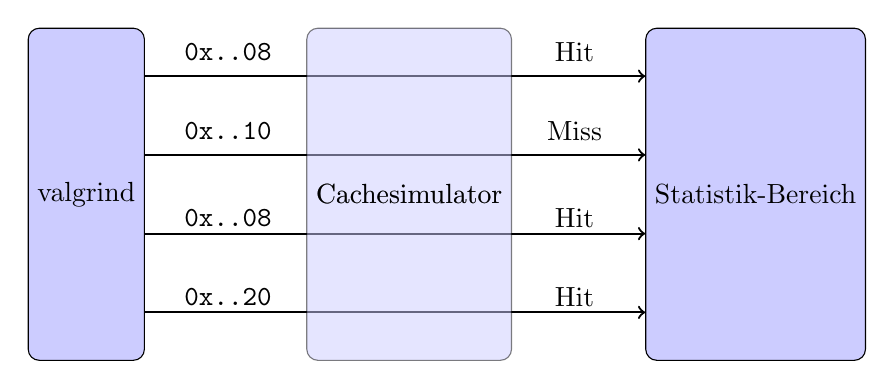
\begin{tikzpicture}
			\node [block,minimum height=120] (valg) at (0,0) {valgrind};
			\node [block,minimum height=120] (stat) at (8.5,0) {Statistik-Bereich};
			\path [draw,->,thick] ([yshift=1.5cm]valg.east) -- ([yshift=1.5cm]stat.west);
			\path [draw,->,thick] ([yshift=0.5cm]valg.east) -- ([yshift=0.5cm]stat.west);
			\path [draw,->,thick] ([yshift=-0.5cm]valg.east) -- ([yshift=-0.5cm]stat.west);
			\path [draw,->,thick] ([yshift=-1.5cm]valg.east) -- ([yshift=-1.5cm]stat.west);
			\node [block,minimum height=120,opacity=0.5] (csim) at (4.1,0) {Cachesimulator};
			\node at (4.1,0) {Cachesimulator};
			\node at (1.8,-1.3cm) {\texttt{0x..20}};
			\node at (1.8,-0.3cm) {\texttt{0x..08}};
			\node at (1.8,0.8cm) {\texttt{0x..10}};
			\node at (1.8,1.8cm) {\texttt{0x..08}};
			\node at (6.2,-1.3cm) {Hit};
			\node at (6.2,-0.3cm) {Hit};
			\node at (6.2,0.8cm) {Miss};
			\node at (6.2,1.8cm) {Hit};
		\end{tikzpicture}
	%\end{block}
\end{frame}

\begin{frame}{Cachesimulator}
	\begin{block}{Cachesimulator}
		\begin{itemize}[<+->]
			\item mengenassoziativ
			\item Realisiert über ein Array aus Tags
			\item Tag gibt zu einer Cachezelle die gecachteSpeicheradresse an
			\item Mehrere nebeneinanderliegende Tags werden zu einem Set zusammengefasst
			\item Bei einem Speicherzugriff wird die Speicheradresse in ein Set abgebildet
			\item Alle Tags dieses Sets werden überprüft, bei einer Übereinstimmung handelt es sich um einen Hit
			\item Bei einem miss wird der Tag des Zugriffs an den anfang des Sets geschrieben und alle anderen nach hinten verdrängt
		\end{itemize}
	\end{block}
\end{frame}

\begin{frame}{Statistik-Bereich}
	\begin{tikzpicture}
		\node [cloud] (accev) {Speicherzugriffe};
		\pause
		\node [block, below of=accev] (calc) {Reverse Adressrechnung};
		\path [draw,->] (accev) -- (calc);
		\node [cloud] (absstat) at (5.7,-1.7) {Zugriffe pro Matrix-Zelle};
		\node [cloud] (relstat) at (5.7,-2.6) {Statistik: Relative Zugriffe};
		\path [draw,->] (calc) -- (absstat.west);
		\path [draw,->] (calc) -- (relstat.west);
		\pause
		\node [cloud, below of=calc] (raccv) {Relative Zugriffe};
		\path [draw] (calc) -- (raccv);
		\node [block, below of=raccv] (patseq) {Pattern/Sequence-Logik};
		\path [draw,->] (raccv) -- (patseq);
		\node [cloud] (pat) at (5.7,-5.0) {Zugriffe pro Matrix-Zelle};
		\node [cloud] (seq) at (5.7,-5.9) {Statistik: Relative Zugriffe};
		\path [draw,->] (patseq.north east) -- (pat.west);
		\path [draw,->] (patseq) -- (seq.west);
	\end{tikzpicture}
\end{frame}

\subsection{Dateiformat} \subsection{Introduction}

Firstly I'd like to state that we are closely following the GZIP file format specification version 4.3 (as found at http://www.gzip.org/zlib/rfc-gzip.html) in structure, design and sometimes content.

\paragraph{Purpose}

The purpose of this specification is to define a byte-oriented data format that can save all of the statistical data collected by the valgrind tool McTracer. Specifically that means that it's able to save
the data collected for several diffrent matrices into one file. The data for one matrix consists of information about individual matrix elements, relative accesses, access patterns and access sequences as
well as some statistical data about the matrix as a whole.

\paragraph{Intended audience}

This specification is intended for use by implementors of software to read the etis format and display it in a way that makes it easier to understand by humans.

The text of the specification assumes a background in programming at the level of bits and other primitve data representations.

\paragraph{Changes from previous versions}
Currently we are at Version 3. Version 1 was bascially a draft, outlining the ideas behind the format for the first time. Version 2 improved the general design and made changes to some field-sizes. 
In Version 3 support for patterns and sequences was added.

\subsection{Detailed Specification} \subsubsection{Overall conventions}

In the diagrams below, a box like this:
\begin{verbatim}
+---+
|   | <-- the vertical bars might be missing
+---+
\end{verbatim}
represents one byte; a box like this:
\begin{verbatim}
+==============+
|              |
+==============+
\end{verbatim}
represents a variable number of bytes.

Within a computer, a number may occupy multiple bytes. All multi-byte numbers in the format described here are 
stored with the least-significant byte first (at the lower memory address). For example, the decimal number 520 
is stored as:
\begin{verbatim}
    0        1
+--------+--------+
|00001000|00000010|
+--------+--------+
 ^        ^
 |        |
 |        + more significant byte = 2 x 256
 + less significant byte = 8
\end{verbatim}

All values are unsigned unless noted otherwise.

\subsubsection{File Format}

An etis file consists of a file-header, a cluster of matrice-headers and a number of matrix data blocks (MDB). 
The header formats and the format of the MDBs will be specified in the following sections.

\paragraph{File-Header (FH) 4 Byte}$\;$ \\

The file header has the following structure:

\begin{verbatim}
+---+---+---+---+
|ID1|ID2| V |NM |
+---+---+---+---+
\end{verbatim}
ID1 (IDentification 1) 1 Byte \\
ID2 (IDentification 2) 1 Byte
\begin{addmargin}[0,5cm]{0,5cm} 
	These have fixed values ID1 = 175 (0xaf, \textbackslash0257), ID2 = 254 (0xfe, \textbackslash0376), to identify the file as being in etis format.
\end{addmargin} 
V (Version) 1 Byte
\begin{addmargin}[0,5cm]{0,5cm} 
	Specifies the version of the fileformat that the current file is in. Currently at 3.
\end{addmargin}
NM (Number of Matrices) 1 Byte
\begin{addmargin}[0,5cm]{0,5cm} 
	The overall number of traced matrices.
\end{addmargin}

\paragraph{Matrix Header (MH) 36 Byte}$\;$ \\

Exactly FH:NM matrix header simply appear one after another in the file, with no additional information 
before, between, or after them.
\begin{verbatim}
+---+---+---+---+---+---+---+---+---+---+---+---+---+---+---+---+
|  SX   |  SY   |NLA|NSA|NAP|NSQ|              ADR              |
+---+---+---+---+---+---+---+---+---+---+---+---+---+---+---+---+
|     MDBADR    |     SLH       |      SLM      |      SSH      |
+---+---+---+---+---+---+---+---+---+---+---+---+---+---+---+---+
|      SSM      |
+---+---+---+---+
\end{verbatim}
SX (Size X) 2 Byte (signed!)
\begin{addmargin}[0,5cm]{0,5cm} 
	The size of the matrix in x direction (number of columns). Must be positive.
\end{addmargin}
SY (Size Y) 2 Byte (signed!)
\begin{addmargin}[0,5cm]{0,5cm} 
	The size of the matrix in y direction (number of rows). Must be positive.
\end{addmargin}
NLA (Number of Loading Accesses) 1 Byte
\begin{addmargin}[0,5cm]{0,5cm} 
	The number of saved relative accesses loading data from this matrix. Maximum of eight.
\end{addmargin}
NSA (Number of Storing Accesses) 1 Byte
\begin{addmargin}[0,5cm]{0,5cm} 
	The number of saved relative accesses storing data into this matrix. Maximum of eight.
\end{addmargin}
NAP (Number of Accesss Patterns) 1 Byte
\begin{addmargin}[0,5cm]{0,5cm} 
	The number of access patterns saved for this matrix.
\end{addmargin}
NSQ (Number of access SeQuences) 1 Byte
\begin{addmargin}[0,5cm]{0,5cm} 
	The number of access sequences saved for this matrix.
\end{addmargin}
ADR (ADRess) 8 Byte $\rightarrow$ 64-Bit
\begin{addmargin}[0,5cm]{0,5cm} 
	The pointer of the matrix.
\end{addmargin}
MDBADR (MDB ADRess) 4 Byte
\begin{addmargin}[0,5cm]{0,5cm} 
	The adress of the affiliated MDB in this file.
\end{addmargin}
SLH (Sum Load Hits) 4 Byte
\begin{addmargin}[0,5cm]{0,5cm} 
	The sum of all load hits for this matrix.
\end{addmargin}
SLM (Sum Load Misses) 4 Byte
\begin{addmargin}[0,5cm]{0,5cm} 
	The sum of all load misses for this matrix.
\end{addmargin}
SSH (Sum Store Hits) 4 Byte
\begin{addmargin}[0,5cm]{0,5cm} 
	The sum of all store hits for this matrix.
\end{addmargin}
SSM (Sum Store Misses) 4 Byte
\begin{addmargin}[0,5cm]{0,5cm}
	The sum of all store misses for this matrix.
\end{addmargin}

\paragraph{Matrix Data Block (MDB)}$\;$ \\

A Matrix Data Block consists of two byte arrays, some (MH:NLA+MH:NSA) relative accesses, some (MH:NAP) access 
patterns, several (MH:NSQ) access sequences and the name assigned to the matrix.

\subparagraph{2 x Byte Array (BA) (MH:SX * MH:SY) Byte}$\;$ \\

One byte array has a size of MH:SX*MH:SY and every byte signifies one matrix element. The matrix is traversed 
row by row. The first byte array represents the tracked load accesses, the second one the store accesses. 
The value of each byte signifies the hit to miss ratio of accesses to the specific element. 
A value of 0 signifies 0\% hits (only misses) and a value of 254 signifies 100\% hits. 
The value 255 is reserved to show that there wasn't any access to this element.

\subparagraph{Relative Access (RA) 12 Byte}$\;$ \\

First there are all MH:NLA different relative accesses for loading from the matrix, then the MH:NSA diffrent 
relative accesses for storing into the matrix. They simply appear one after another in the file, with no 
additional information before, between, or after them.
\begin{verbatim}
+---+---+---+---+---+---+---+---+---+---+---+---+
|  OX   |  OY   |      SH       |      SM       |
+---+---+---+---+---+---+---+---+---+---+---+---+
\end{verbatim}
OX (Offset X) 2 Byte (signed!)
\begin{addmargin}[0,5cm]{0,5cm} 
	The x offset of this relative access.
\end{addmargin}
OY (Offset Y) 2 Byte (signed!)
\begin{addmargin}[0,5cm]{0,5cm} 
	The y offset of this relative access.
\end{addmargin}
SH (Sum of Hits) 4 Byte
\begin{addmargin}[0,5cm]{0,5cm} 
	The accumulated number of hits for this type of relative access.
\end{addmargin}
SM (Sum of Misses) 4 Byte
\begin{addmargin}[0,5cm]{0,5cm} 
	The accumulated number of misses for this type of relative access.
\end{addmargin}
\newpage
\subparagraph{Access Pattern (AP) 7 Byte + AP:LEN * 12 Byte}$\;$ \\

An access pattern combines a series of relative accesses. There are exactly MH:NAP different access patterns
 one after another. Each pattern consists of a short pattern header and afterwards AP:LEN diffrent relative 
accesses as defined above. They simply appear one after another in the file, with no additional information 
before, between, or after them.
\begin{verbatim}
+---+---+---+---+---+---+---+
|ID |      SO       |  LEN  |
+---+---+---+---+---+---+---+
\end{verbatim}
ID (IDentification) 1 Byte
\begin{addmargin}[0,5cm]{0,5cm} 
	An identification number that is unique in the context of the current matrix.
\end{addmargin}
SO (Sum of Occurences) 4 Byte
\begin{addmargin}[0,5cm]{0,5cm} 
	The accumulated sum of occurences of this pattern.
\end{addmargin}
LEN (LENgth) 2 Byte
\begin{addmargin}[0,5cm]{0,5cm} 
	The length of this pattern.
\end{addmargin}
	
\subparagraph{Access Sequence (SQ) 12 Byte}$\;$ \\

An access sequence consists of uninterrupted repetitions of a pattern combined with the next access or next 
pattern. There are exactly MH:NSQ diffrent sequences one after another. They simply appear one after another 
in the file, with no additional information before, between, or after them.
\begin{verbatim}
+---+---+---+---+---+---+---+---+---+---+---+---+
|PID|      SO      |   RP   |  NX   |  NY   |NID|
+---+---+---+---+---+---+---+---+---+---+---+---+
\end{verbatim}
PID (Pattern IDentification) 1 Byte
\begin{addmargin}[0,5cm]{0,5cm} 
	The AP:ID of the pattern that is repeated.
\end{addmargin}
SO (Sum of Occurences) 4 Byte
\begin{addmargin}[0,5cm]{0,5cm} 
	The accumulated sum of occurrences of this sequences
\end{addmargin}
RP (RePetitions) 2 Byte
\begin{addmargin}[0,5cm]{0,5cm} 
	The number of uninterrupted repetitions of the pattern.
\end{addmargin}
NX (Next access offset X) 2 Byte (signed!)
\begin{addmargin}[0,5cm]{0,5cm} 
	The x offset of the access following the sequence.
\end{addmargin}
NY (Next access offset Y) 2 Byte (signed!)
\begin{addmargin}[0,5cm]{0,5cm} 
	The y offset of the access following the sequence.
\end{addmargin}
NID (Next IDentification) 1 Byte
\begin{addmargin}[0,5cm]{0,5cm} 
	References the pattern following the sequence. 0xff if none could be found.
\end{addmargin}

\subparagraph{Name (NA)}$\;$ \\
\begin{verbatim}
+========+
|  NAME  |
+========+
\end{verbatim}
NAME (Name) Null terminated
\begin{addmargin}[0,5cm]{0,5cm} 
	The name of the matrix, as it's passed when the tracing starts. ASCII-encoded.
\end{addmargin}


\subsection{Overview}
\includegraphics[width=\textwidth]{fileformat/structure}
This is a conceptual outline of an etis file. It consists of the file header, three matrix headers and three matrix data blocks (MDB). The first MDB is then displayed in more detail to show the diffrent element
that it contains, namely namely two byte arrays, several relative accesses, three patterns with one, one and three sequences and the name. The last detail shows an access pattern in some more detail.